
%******Average number of frame loss event******
\begin{figure*}[!t]
	%\begin{figure*}[t]
	\centering
	\subfigure[Average Number Of Frame Loss Event]  {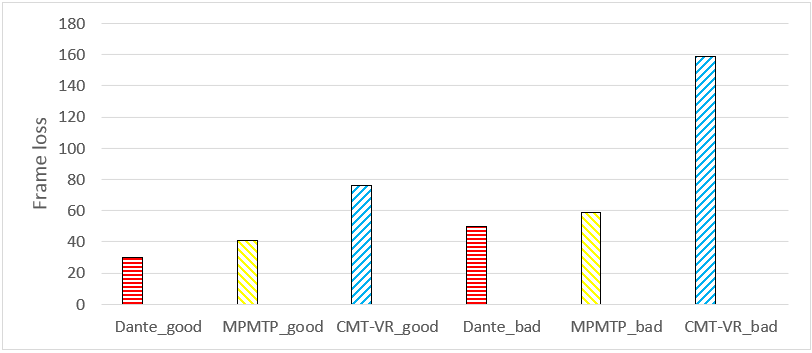
\includegraphics[width=8cm,angle=0]{paper_figs/evaluation_result/sub/frameLoss.png}}
	\subfigure[Multiple Metrics Of Video Quality]  {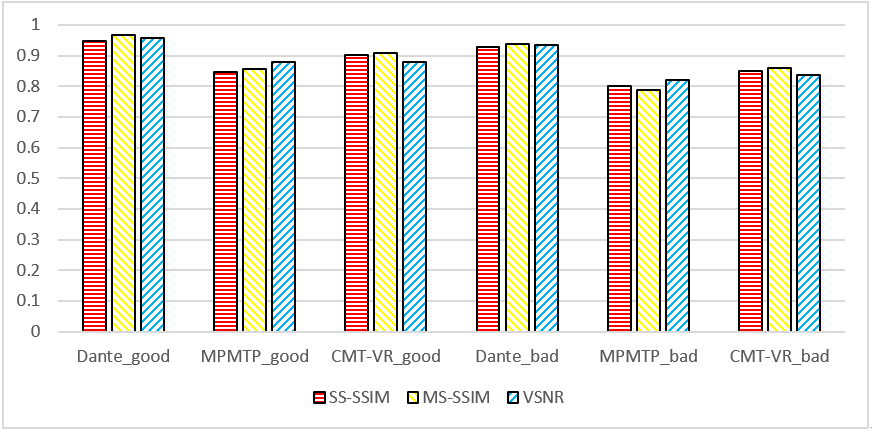
\includegraphics[width=8cm,angle=0]{paper_figs/evaluation_result/sub/multi_metrics.png}}
	\vspace{-0.3cm}
	\caption{Average Frame Loss Number And Multiple Metrics For video Quality In Good And Bad Network Condition}
	\vspace{-0.4cm}
	\label{fig:apuct}
\end{figure*}


%*****Instantaneous PSNR In relatively Bad Network Condition*****	

\begin{figure*}[!t]
	%\begin{figure*}[t]
	\centering
	\subfigure[Video Sequence 1]  {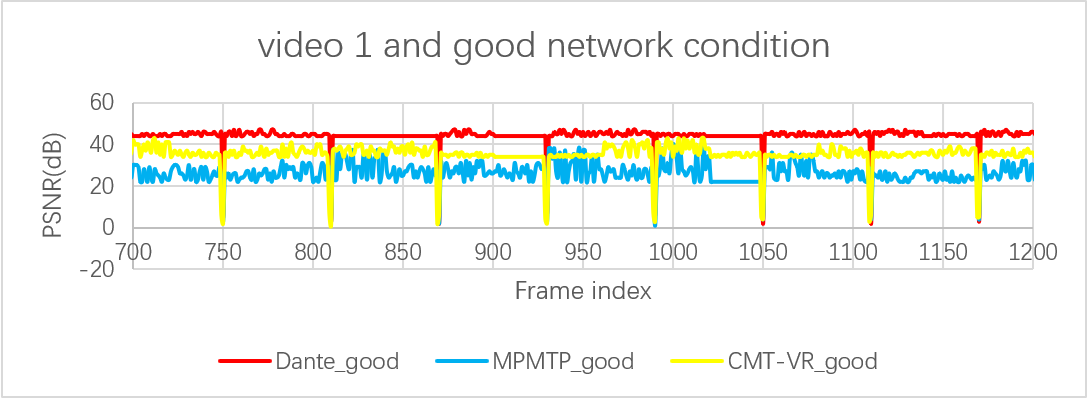
\includegraphics[scale=0.175,angle=0]{paper_figs/evaluation_result/sub/ins_psnr_v1_good.png}}
	\subfigure[Video Sequence 2]  {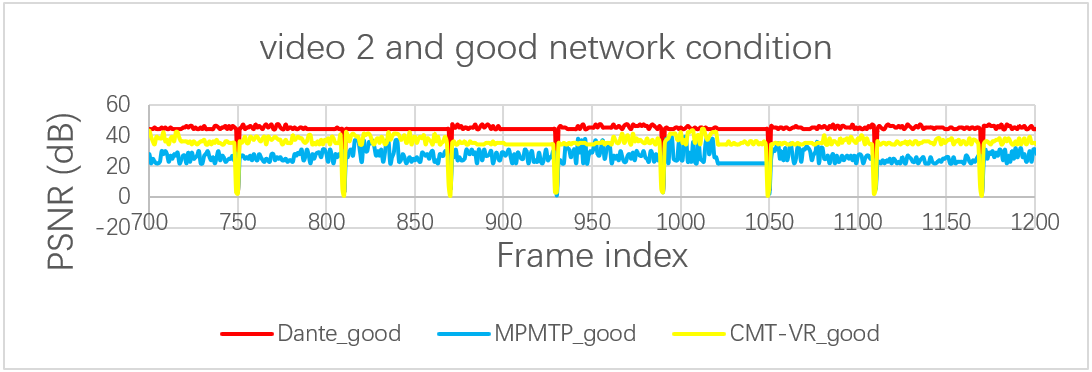
\includegraphics[scale=0.19,angle=0]{paper_figs/evaluation_result/sub/ins_psnr_v2_good.png}}
	\subfigure[Video Sequence 3]  {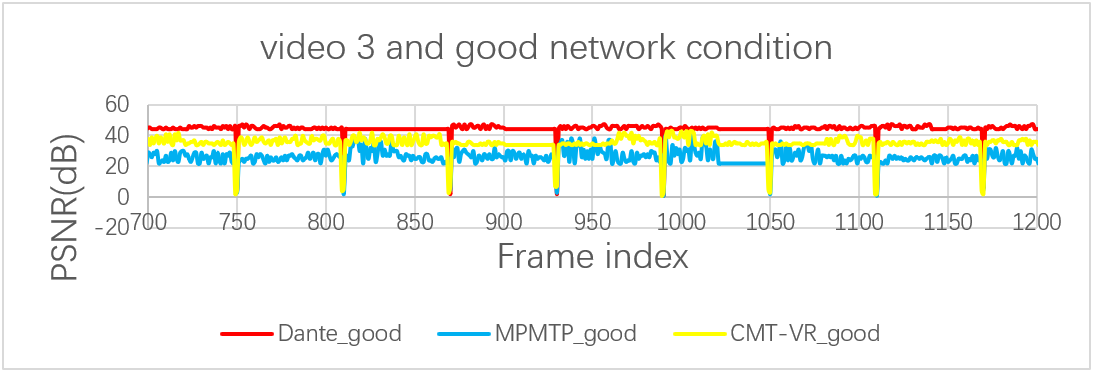
\includegraphics[scale=0.19,angle=0]{paper_figs/evaluation_result/sub/ins_psnr_v3_good.png}}
	\vspace{-0.3cm}
	\caption{Instantaneous PSNR In Relatively Good Network Condition}
	\vspace{-0.4cm}
	\label{fig:apuct}
\end{figure*}

%*****Instantaneous PSNR In relatively Good Network Condition*****
\begin{figure*}[!t]
	%\begin{figure*}[t]
	\centering
	\subfigure[Video Sequence 1]  {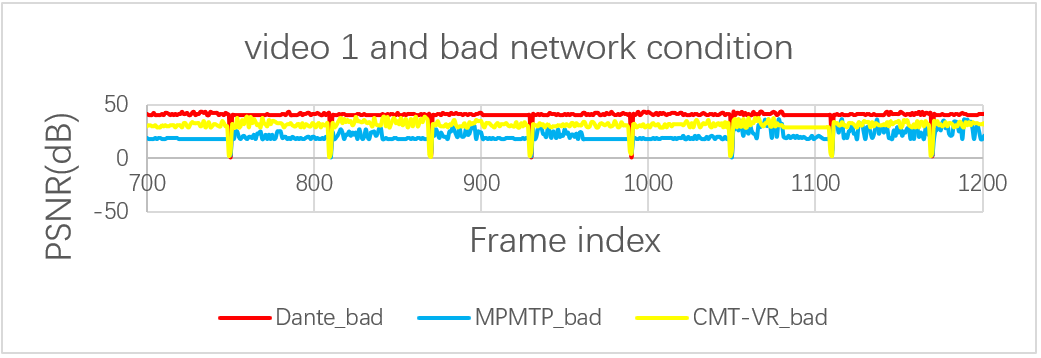
\includegraphics[scale=0.205,angle=0]{paper_figs/evaluation_result/sub/ins_psnr_v1_bad.png}}
	\subfigure[Video Sequence 2]  {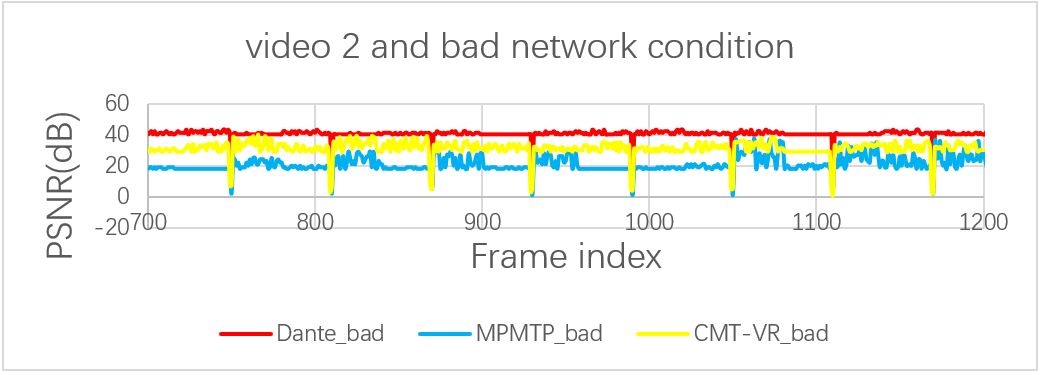
\includegraphics[scale=0.195,angle=0]{paper_figs/evaluation_result/sub/ins_psnr_v2_bad.png}}
	\subfigure[Video Sequence 3]  {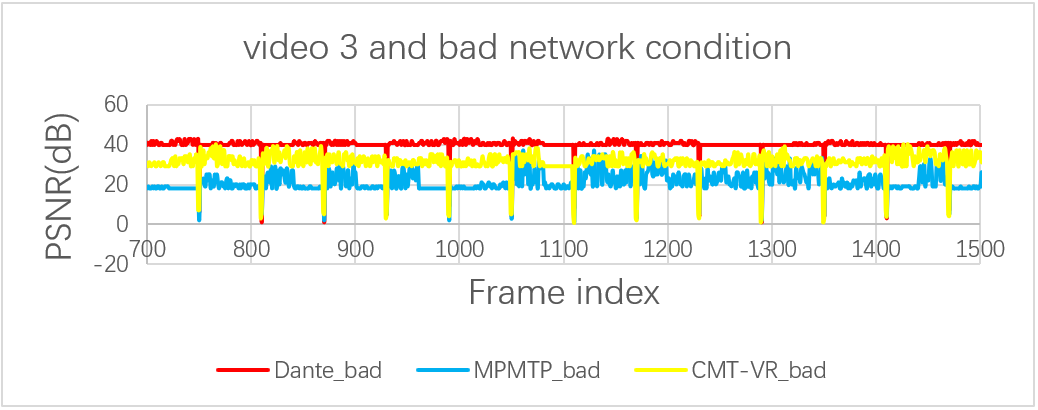
\includegraphics[scale=0.18,angle=0]{paper_figs/evaluation_result/sub/ins_psnr_v3_bad.png}}
	\vspace{-0.3cm}
	\caption{Instantaneous PSNR In Relatively Bad Network Condition}
	\vspace{-0.4cm}
	\label{fig:apuct}
\end{figure*}	

%*****Culmulative Distribution Function Of PSNR In relatively good Network Condition*****	
\begin{figure*}[!t]
	%\begin{figure*}[t]
	\centering
	\subfigure[Video Sequence 1]  {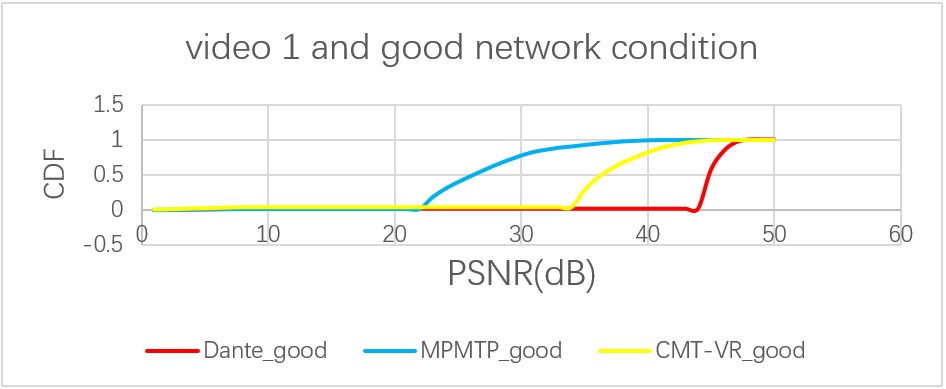
\includegraphics[scale=0.21,angle=0]{paper_figs/evaluation_result/sub/cdf_v1_good.png}}
	\subfigure[Video Sequence 2]  {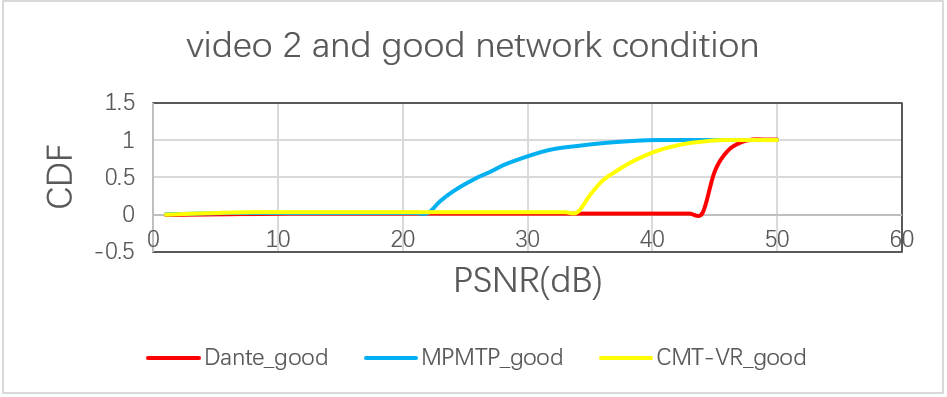
\includegraphics[scale=0.20,angle=0]{paper_figs/evaluation_result/sub/cdf_v2_good.png}}
	\subfigure[Video Sequence 3]  {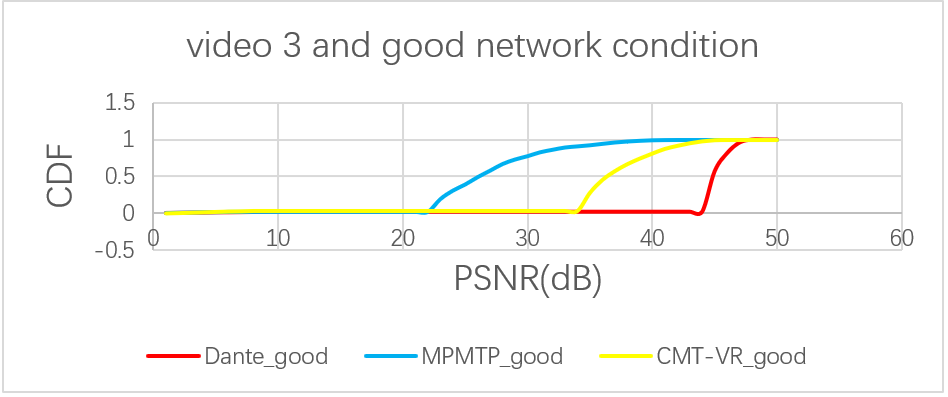
\includegraphics[scale=0.205,angle=0]{paper_figs/evaluation_result/sub/cdf_v3_good.png}}
	\vspace{-0.3cm}
	\caption{Culmulative Distribution Function Of PSNR In Relatively Good Network Condition}
	\vspace{-0.4cm}
	\label{fig:apuct}
\end{figure*}


%*****Culmulative Distribution Function Of PSNR In relatively Bad Network Condition*****		
\begin{figure*}[!t]
	%\begin{figure*}[t]
	\centering
	\subfigure[Video Sequence 1]  {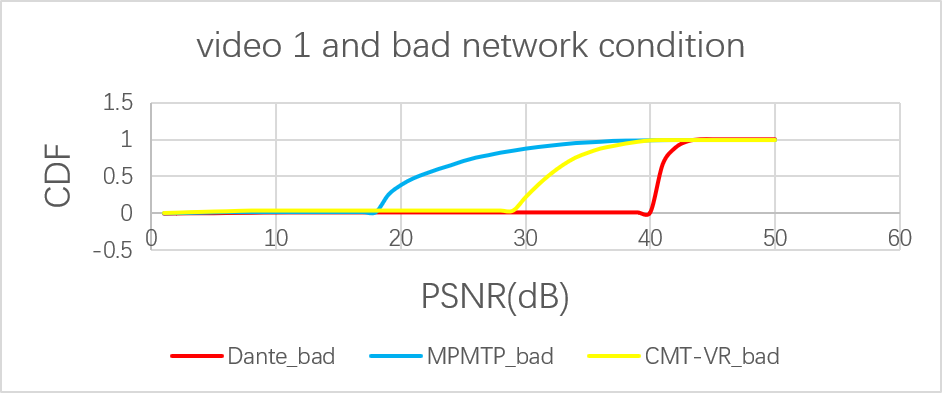
\includegraphics[scale=0.21,angle=0]{paper_figs/evaluation_result/sub/cdf_v1_bad.png}}
	\subfigure[Video Sequence 2]  {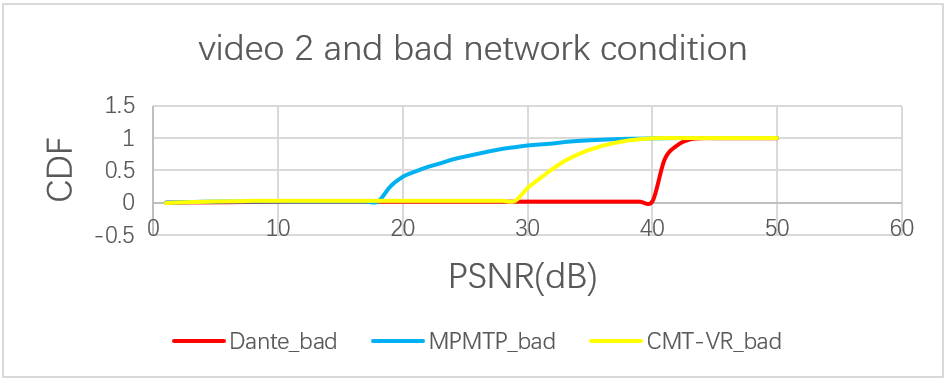
\includegraphics[scale=0.195,angle=0]{paper_figs/evaluation_result/sub/cdf_v2_bad.png}}
	\subfigure[Video Sequence 3]  {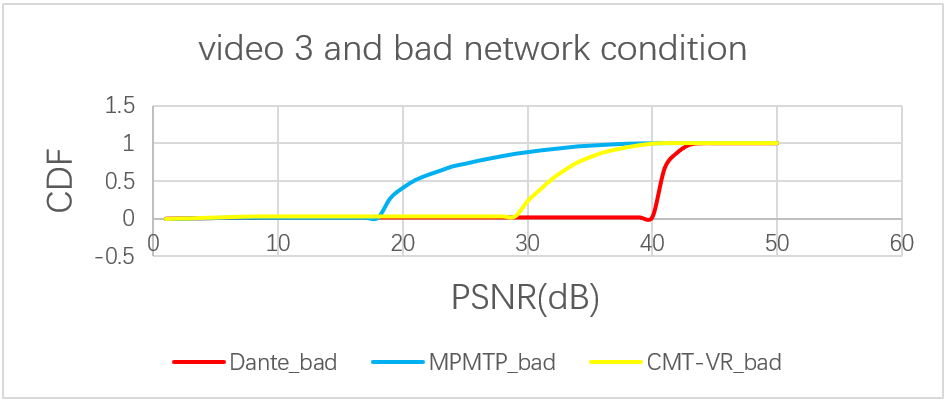
\includegraphics[scale=0.19,angle=0]{paper_figs/evaluation_result/sub/cdf_v3_bad.png}}
	\vspace{-0.3cm}
	\caption{Culmulative Distribution Function Of PSNR In Relatively Bad Network Condition}
	\vspace{-0.4cm}
	\label{fig:apuct}
\end{figure*}	





\section{Performance Evaluation}
We conducted extensive experiments to demonstrate Dante performance gains on QoE. Specifically, the evaluation metrics considered in this work include single scale and multi-scale structural similarity(SS-SSIM and MS-SSIM), Signal-to-Noise Ratio(VSNR), PSNR and frame loss frequency. 

\subsection{Experimental Set-up}
\textbf{Experiment topology:} 5 sources connect to node N0, while 5 sinks connect to node N1. And N0 connects to N1 through two lossy links. Sources and sinks represent servers and clients respectively, and Dante is deployed on all servers and clients. The topology is not shown because of space limitation. The experiment scenario is that sources send the data to sinks through two lossy links with the request of video segmentations.

\textbf{Testbed configuration:} The sources and sinks are commodity servers with Ubuntu 16.4 (kernel 4.40), each of which is equipped with an Intel(R) Core(TM) i3-4150k cpu @ 3.5GHz (4 cores), two Intel 82599ES 10G dual port NICs and 32 G memory.


\textbf{360-degree video content preparations:} We download three 8K video sequences from Youtube, each of which is transcoded into three kinds of bitrate, such as 50Mbps, 12Mbps and 3Mbps, and then cut into 60 video segmentations with 1s length. In this way, we can get 180 files for every video sequence. At the last step, we utilize 360transformation \cite{360Transformations} to crop spatially each of these files into three layers including the QER layer, cushion layer and outmost layer, and total 540 video representations for every video are obtained. All files of video segmentations are preprocessed, generated and managed on the server side.\\
\textbf{Network parameter set:} Gilbert model is adopted to mimic the packet loss pattern in real wireless networks, supported by traffic control (TC)~\cite{TC}, in which four parameters($\xi _i^G$, $\xi _i^B$, 1-h and 1-k) are needed, $\xi _i^G$ and $\xi _i^B$ are transition probabilities between the bad and good state, 1-h and 1-k is the loss probability in the bad state and good state, respectively. In our testbed, 1-h and 1-k are set as 1 and 0, respectively. Meanwhile, average packet loss rate is equal to $\pi _i^B = \xi _i^B/(\xi _i^B\\ + \xi _i^P)$. And the bandwidth of two path is set randomly in corresponding specified range and RTT is set as 50ms and 100ms for Path-A and Path-B, respectively. Detailed Parameter set is seen in Table 2. 

\begin{table}
	\centering 
	\scriptsize
	\begin{tabular}{cp{0.95cm}p{1.6cm}p{0.8cm}p{2.0cm}}
		\rowcolor[gray]{0.9} 
		\hline
		(A) Network &  Time(Sec.)    & Bandwidth(Mbps)       &  RTT(ms) &  Pakcet loss rate(\%) \\
		\hline
		Path-A  &  0${\sim}$20   &  15${\sim}$40         &     50   &  $\xi _i^B$ = 0.03, $\xi _i^G$ = 10\\
		
		Path-A  &  20${\sim}$40  &  15${\sim}$40         &     50   &  $\xi _i^B$ = 0.05, $\xi _i^G$ = 10\\ 
		
		Path-A  &  40${\sim}$60  &  15${\sim}$40         &     50   &  $\xi _i^B$ = 0.1,  $\xi _i^G$ = 10\\   
		
		Path-B  &  0${\sim}$20   &  10${\sim}$20         &     100  &  $\xi _i^B$ = 0.05, $\xi _i^G$ = 10\\
		
		Path-B 	&  20${\sim}$40  &  10${\sim}$20         &     100  &  $\xi _i^B$ = 0.1,  $\xi _i^G$ = 10\\	
		
		Path-B 	&  40${\sim}$60  &  10${\sim}$20         &     100  &  $\xi _i^B$ = 0.3,  $\xi _i^G$ = 10\\  	
		
		\hline
		\rowcolor[gray]{0.9}
		\hline
		(B) Network &   Time(Sec.)   & Bandwidth(Mbps)       &  RTT(ms) &     Pakcet loss rate(\%)  \\
		
		Path-A  &  0${\sim}$20   &  15${\sim}$40         &    50    &  $\xi _i^B$ = 0.05, $\xi _i^G$ = 10\\
		
		Path-A  &  20${\sim}$40  &  15${\sim}$40         &    50    &  $\xi _i^B$ = 0.1,  $\xi _i^G$ = 10\\ 
		
		Path-A  &  40${\sim}$60  &  15${\sim}$40         &    50    &  $\xi _i^B$ = 0.2,  $\xi _i^G$ = 10\\     
		
		Path-B  &  0${\sim}$20   &  10${\sim}$20         &    100   &  $\xi _i^B$ = 0.15, $\xi _i^G$ = 10\\
		
		Path-B  &  20${\sim}$40  &  10${\sim}$20         &    100   &  $\xi _i^B$ = 0.3,  $\xi _i^G$ = 10\\	
		
		Path-B  &  40${\sim}$60  &  10${\sim}$20         &    100   &  $\xi _i^B$ = 0.5,  $\xi _i^G$ = 10\\ 
		
		\hline
		
	\end{tabular}
	\caption{Network Condition of Two Wireless networks: (A)Relatively Good Wireless Conditions And (B)Relatively Bad Wireless Conditions}
	\label{}
\end{table}



\subsection{Performance Comparison With Existing Protocols}
We consider MPMTP~\cite{MPMTP}, content-agnostic, and CMT-VR~\cite{CMT-VR}, content-aware,  as reference schemes, both of which utilize Raptor codes to guarantee reliability, mitigating the unnecessary retransmissions.	

First, as show in Figure 5.a, Dante encounters the minimum times of frame loss event no matter in relatively good or bad network condition. Meanwhile, to demonstrate the perceived 360 degree video quality, Figure 5.b gives a group of results from multiple metrics including SS-SSIM, MS-SSIM and VSNR, we can see that Dante, compared with MPMTP and CMT-VR, better performs in subjective video quality in good network status or relatively bad network status.     
Then, Figure 6 and Figure 7 compare instantaneous PSNR of three video sequences in good network condition and bad network condition, respectively. The result shows that Dante achieves a great improvement of PSNR, compared to MPMTP and CMT-VR. The reason why MPMTP performs worst in all protocols is that, despite no involving retransmissions and maximizing the throughput, it doesn't consider video's inherent feature, such as decoding dependencies of video codec, which should have give different frame unequal attention, and thus can't utilize effectively the network allocation to boost video quality. Meanwhile, CMT-VR performs better than MPMTP, due to its consideration of frame priority. However, unfortunately, non-FOV-aware reliability scheme makes it waste valuable bandwidth on trival data, thus CMT-VR is the secondary one. Dante takes into acount not only traditional video features aforementioned, but FOV. Benefiting from the hierarchical protection spatially and temporally, Dante achieves desirable upgrade in instantaneous PSNR and cultimulative distribution function of PSNR shown in Figure 8 and Figure 9.  	         
